\begin{figure*}[t]
    \centering
    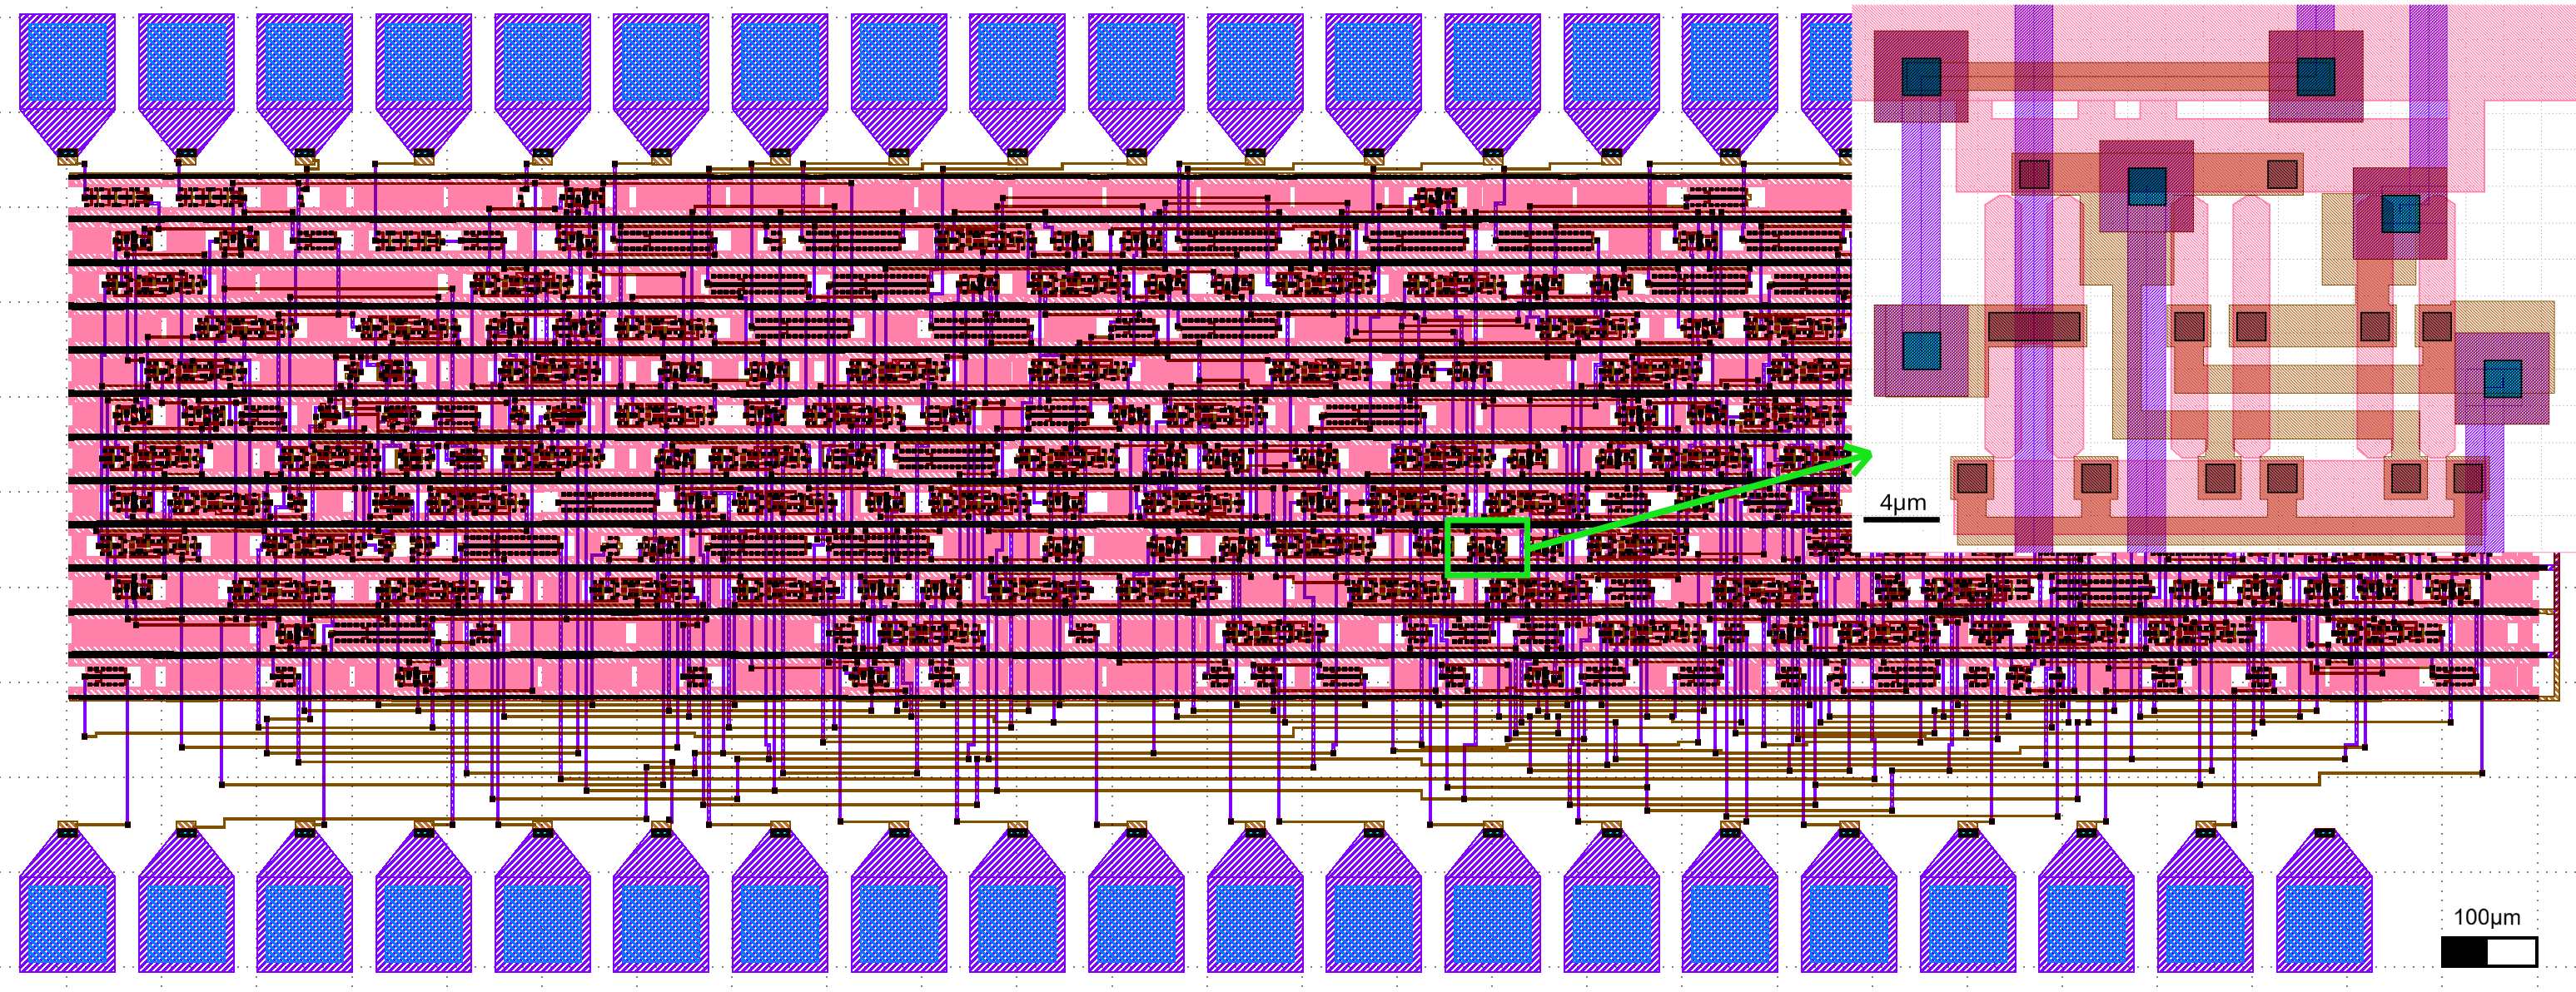
\includegraphics[width=0.6\textwidth]{Core.png}
    \label{fig:Core}
    \caption{A digital core made in AMF silicon photonics technology. It has two 12-bits wide pads for ADC/DAC connections. }
\end{figure*}
As recent state-of-the art shows, MOSFET transistor in a conventional silicon photonics node can be useful for power reading applications and signal multiplexing\CitationNeeded. 
While the design of the basic transistor unit is a promising start, improving the design opens up the possibilities of integrating digital electronics.
This section will present the modeling of the transistors and the effect of the proposed changes has on key parameters; the small signal gain ($gm$) and the cut-off frequency ($F_t$).

The chosen key parameters were selected for their relevance to both the analog and digital circuitry. 
A higher small signal gain means that analog circuitery requires less transistor for the same amplification factor, shrinking the circuits as a whole. 
The increase of the small signal gain also increases the current output strength of digital gates, helping in the charge and discharge of capacitive loads, such as gates or PN junctions. 
The other parameter, the cut-off frequency of the transistor themselves, is a measurment of how fast a single transistor can switch.
Improving the cut-off frequency of the transistor opens up the design area for analog and digital circuitry as it represents the upper limit at which a circuit can run in a parasitic-less environment.  
Improving both these metrics can lead to more precision and efficiency in signal collection and transport.

The saturation region small signal gain is the measurment of how much the drain current ($I_D$) changes in relation with the gate-to-source voltage ($V_{GS}$) in a specific condition of the drain-to-source voltage ($v_{DS}$).

\begin{equation}
\label{eq:gm}
gm = \left.\frac{\delta I_D}{\delta V_{GS}}\right|_{v_{DS}} = \mu_x C_{ox}\frac{W}{L}(V_{GS}-V_T)(1+\lambda v_{DS})
\end{equation}

In \ref{eq:gm}, $\mu_x$ is the mobility of the charges, $C_{ox}$ is the oxide capacitance per unit area, $W$ and $L$ are the size of the gate, $V_T$ is the threshold voltage and $\lambda$ is the channel-length modulation parameter. 
In  conventionnal silicon photonics process, the $W$ value is the height of the waveguide, hence the designer only has access on controlling the bias point via  $V_{GS}$ via an external application, and the length $L$ and the oxide capacitance $C_{ox}$ up to their respective manufacturing limit.
The length of the transistor is controllable by the distance between two tubs of the same type of doping and the length of the gate.
As the physical limit of the gate length is the minimal width of a silicon waveguide, the limiting factor is often the minimal distance between two tubs of similar doping without causing a unwanted connection between the source and the drain.
Depending on the foundry used, this distance can vary and be subject to mask alignment precision. 
As for the $C_{ox}$ value, it is not only found in \ref{eq:gm} but also in the formula of $V_T$, which influences the bias point and $gm$.

\begin{equation}
\label{eq:Vt}
V_T = V_{fb} + 2\phi_F + \frac{\sqrt{2\varepsilon_{Si} qN(2\phi_F)}}{C_{ox}}
\end{equation}

In (\ref{eq:Vt}), $V_{fb}$ is the flat band voltage,  $\phi_F$ is fermi potential of the doped channel, $\varepsilon_{Si}$ the permitivity of silicon, $q$ the elemental charge and $N$ the doping of the channel.
It is better to increase the $C_{ox}$ value as much as possible, as it has the double effect of reducing the $V_T$ in (\ref{eq:Vt}) and increasing the $gm$ from (\ref{eq:gm}).

The second metric, the cut-off frequency $F_T$, it's small-signal gain over its gate-source ($C_{GS}$) and gate-drain capacitance ($C_{GD}$) %\cite{Sedra2014}.

\begin{equation}
\label{eq:Ft}
F_t = \frac{gm}{2\pi(C_{GS}+C_{GD})} = \frac{\mu_x(V_{GS}-V_t)}{2\pi (\frac{2}{3}L^2+2L_{ov}L)},
\end{equation}

where $L_{ov}$ the overlap length between the gate and the source or drain area.

In the litterature, a $V_t$ of around 2$V$ was achieved using larger than minimal values of $L$ and $C_{ox}$\CitationNeeded. 
This $V_T$ value could be further improved by shaving away at the gap between the gate and the channel, reducing it from 200 nm to 160 nm or even 140 nm, increasing the $C_{ox}$ value. 
Together with the diminution of the $L$ value, one could increase the maximum frequency of operation by a factor of around 80 to 100 and the $gm$ around\CitationNeeded.

With the improvements made to the basic MOSFET, the next step is to create a analog and digital library of circuits enabling semi-automated designs. 





